\section{Introduction}

\subsection{Motivation}

Over the last decades the number of transistors on a chip is steadily rising (figure~\ref{fig:moors_law}).
Moore's Law is thereby the observation, that this number doubles roughly every 2 years \cite{moores_law}.
Thus, the amount of functional units per chip rises at the same rate and this trend will probably continue.
This leads to more complex designs.

\begin{figure}[htb]
 \centering
 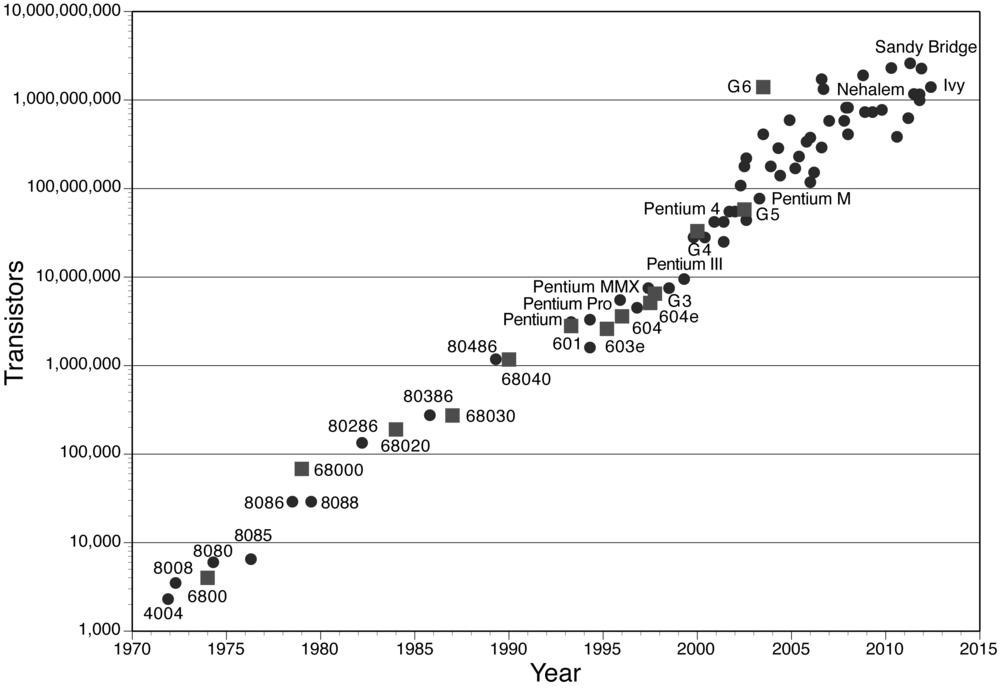
\includegraphics[width=1.0\textwidth,angle=0]{images/moors_law.png}
 \caption{Number of Transistors on a Chip \cite{moore}}
\label{fig:moors_law}
\end{figure}

Since changes in these designs after tape-out are highly expensive, it is necessary to ensure that the functionality of a design is verified pre-silicon.
The Universal Verification Methodology (UVM) was developed for this purpose. 
It is a standardized methodology and provides the ability to verify each individual component of a design separately.
Its components can be reused, when moving up to system level to validate the interaction between the separate modules of the design.
It provides the ability to automatically generate stimuli for a module and has self-checking capabilities to verify the behavior of the design.
Thereby, the various functionalities of the more complex designs can be verified.\\
In this thesis the methodology is used to verify a microcode engine (MCE), that was developed by the Computer Architecture Group at the Institute of Computer
Engineering, Heidelberg University.

\subsection{Outline}

This thesis is divided into the following sections.
Firstly, an overview of the functionalities of the MCE is given. Including the instruction set and how it is executed within the engine.
Following, the engine is analyzed to identify the parts, that have to be considered for verification.
After that, the Universal Verification Methodology is introduced. It is shown, how to create a general testbench using the provided components and its usage for
Metric Driven Verification.
Next, the structure and functionality of the testbench is shown, which is used to verify the MCE.
Finally, the conclusion is presented and topics for future work are discussed.
